%%%%%%%%%%%%%%%%%%%%%%%%%%%%%%%%%%%%%%%%%%%%%%%%%%%%%%%%%%%%%%%%%%%%%%%%%%%%%%%%
% This is just an example/guide for you to refer to when submitting manuscripts
% to Frontiers, it is not mandatory to use Frontiers .cls files nor
% frontiers.tex  % This will only generate the Manuscript, the final article
% will be typeset by Frontiers after acceptance.
%                                              %
%                                              %
% When submitting your files, remember to upload this *tex file, the pdf
% generated with it, the *bib file (if bibliography is not within the *tex) and
% all the figures.
%%%%%%%%%%%%%%%%%%%%%%%%%%%%%%%%%%%%%%%%%%%%%%%%%%%%%%%%%%%%%%%%%%%%%%%%%%%%%%%%

%%% Version 3.3 Generated 2016/11/10 %%%
%%% You will need to have the following packages installed: datetime, fmtcount,
%etoolbox, fcprefix, which are normally inlcuded in WinEdt. %%%
%%% In http://www.ctan.org/ you can find the packages and how to install them,
%if necessary. %%%
%%%  NB logo1.jpg is required in the path in order to correctly compile front
%page header %%%

\documentclass[utf8]{frontiersSCNS}
\usepackage{url,hyperref,lineno,microtype,subcaption}
\usepackage[onehalfspacing]{setspace}

\linenumbers

\def\keyFont{\fontsize{8}{11}\helveticabold }
\def\firstAuthorLast{Anderson {et~al.}} %use et al only if is more than 1 author
\def\Authors{Sean M. Anderson\,$^{1,*}$, Bernardo S. Mendoza\,$^{1}$}
\def\Address{$^{1}$Centro de Investigaciones en \'Optica, A.C., Le\'on, Mexico}
\def\corrAuthor{Sean M. Anderson\\Centro de Investigaciones en \'Optica, A.C.,
Loma del Bosque 115, Le\'on, 37150, Mexico}

\def\corrEmail{sma@cio.mx}



\begin{document}
\onecolumn
\firstpage{1}

\title[Depth dependent three-layer model for the SSHG yield]
{Depth dependent three-layer model for the surface second-harmonic generation
yield}

\author[\firstAuthorLast ]{\Authors} %This field will be automatically populated
\address{} %This field will be automatically populated
\correspondance{} %This field will be automatically populated

\extraAuth{}


\maketitle


\begin{abstract}
\section{}
We present a generalization of a three-layer model to calculate the surface
second harmonic generation (SSGH) yield, that includes the depth dependence of
the surface nonlinear second order susceptibility tensor
$\boldsymbol{\chi}(-2\omega;\omega,\omega)$. This model considers that the
surface is represented by three regions or layers. The first layer is the vacuum
region with a dielectric function $\epsilon_{v}(\omega)=1$ from where the
fundamental electric field impinges on the material. The second layer is a thin
layer ($\ell$) of thickness $d$ characterized by a dielectric function
$\epsilon_{\ell}(\omega)$, and it is in this layer where the SSHG takes place.
We consider the position of $\boldsymbol{\chi}(-2\omega;\omega,\omega)$ within
this surface layer. The third layer is the bulk region denoted by $b$ and
characterized by $\epsilon_{b}(\omega)$. Both the vacuum and bulk layers are
semi-infinite. The model includes the multiple reflections of both the
fundamental and the second-harmonic (SH) fields that take place at the thin
layer $\ell$. We use the depth dependent three-layer model and compare it
against the experimental results of a Si(111)(1$\times$1):H surface.

\tiny
 \keyFont{ \section{Keywords:} surface, second harmonic generation, SHG, multiple,
 reflections, semiconductor, spectroscopy}
\end{abstract}


\section{Introduction}\label{sec:intro}

Surface second-harmonic generation (SSHG) has been shown to be an effective,
nondestructive and noninvasive probe to study surface and interface properties
\citep{chenPRL81, shenNAT89, mcgilpOE94, bloembergenAPB99, mcgilpSRL99,
lupkeSSR99, downerPSSA01, downerSIA01}. SSHG spectroscopy is now very
cost-effective and popular because it is an efficient method for characterizing
the properties of buried interfaces and nanostructures. The high surface
sensitivity of SSHG spectroscopy is due to the fact that within the dipole
approximation, the bulk second-harmonic generation (SHG) in centrosymmetric
materials is identically zero. The SHG process can occur only at the surface
where the inversion symmetry is broken. SSHG has useful applications for
studying thick thermal oxides on semiconductor surfaces
\citep{vanhasseltJOSAB95, kolthammerPRB05} and thin films \citep{yeganehPRB92}.
The accurate determination of these studies is highly dependent on multiple
reflections of both the SH and fundamental waves in the surface region. These
considerations have been taken into account to study thin films
\citep{haseAPL92, buinitskayaMJPS02, buinitskayaCAS03} and, using the Maker
fringe technique \citep{makerPRL62}, other materials \citep{tellierOC07,
abeJOSAB08}.

\cite{bloembergenPR62} were the first to consider multiple reflections in their
treatment of SHG in a nonlinear slab. However, they only considered the
second-harmonic (SH) fields and derived results for a dielectric with a small
linear reflectance. They also neglected the multiple reflections of the
fundamental waves inside the media. Surface effects were modeled by taking the
limit of a thin slab with a thickness much smaller than the wavelength of the
incoming light. Ref. \citep{dickAPB85} used this methodology to determine the
components of the nonlinear optical susceptibility tensor,
$\boldsymbol{\chi}(-2\omega;\omega,\omega)$, of a fluorescent dye over fused
silica. Later works \citep{sipePRB87, mizrahiJOSA88} developed a simplified
method using phenomenological models in which the surface is treated as an
infinitesimally thin dipole sheet. The inclusion of multiple reflections is
necessary for both the SH radiation and the incoming fundamental fields; this
was experimentally verified in Ref. \citep{moritaJJAP88}, where they show that
the lineshape of the SSHG radiation is composed of resonances from both the SH
and fundamental waves.

As mentioned above, SSHG is particularly useful for studying the surfaces of
centrosymmetric materials. From the theoretical point of view, the calculation
of $\boldsymbol{\chi}(-2\omega;\omega,\omega)$ proceeds as follows. To mimic the
semi-infinite system, we construct a supercell consisting of a finite slab of
material plus a vacuum region. Both the size of the slab and the vacuum region
should be such that the value of $\boldsymbol{\chi}(-2\omega;\omega,\omega)$ is
well converged.  A cut function is used to decouple the two halves of the
supercell in order to obtain the value of
$\boldsymbol{\chi}(-2\omega;\omega,\omega)$ for either half. If the supercell
itself is centrosymmetric, the value $\boldsymbol{\chi}(-2\omega;\omega,\omega)$
for the full supercell is identically zero. Therefore, the cut function is of
paramount importance in order to obtain a finite value for
$\boldsymbol{\chi}(-2\omega;\omega,\omega)$ for either side of the slab
\citep{reiningPRB94,andersonPRB15,andersonPRB16a}. The cut function can be
generalized to one that is capable of obtaining the value of
$\boldsymbol{\chi}(-2\omega;\omega,\omega)$ for any part of the slab. We can
easily obtain the depth within the slab for which
$\boldsymbol{\chi}(-2\omega;\omega,\omega)$ is nonzero; conversely, we can
verify that it goes to zero towards the middle of the slab, where the
centrosymmetry of the material is restored \citep{mejiaRMF04}. Therefore, for
the surface of any centrosymmetric material, we can find the thickness of the
layer where $\boldsymbol{\chi}(-2\omega;\omega,\omega)$ is finite.

Based on this approach for the calculation of
$\boldsymbol{\chi}(-2\omega;\omega,\omega)$, in this paper we generalize the
``three-layer model'' for the SH radiation from the surface of a centrosymmetric
material \citep{andersonPRB16b}. This model considers that the SH conversion
takes place in a thin layer just below the surface of the material that lies
under the vacuum region and above the bulk of the material. It is the
three-layer model that allows us to integrate the effects of multiple
reflections for both the SH and fundamental fields into the SSHG yield. As we
show in this article, this treatment can be generalized to take into account the
\emph{depth} dependence of $\boldsymbol{\chi}(-2\omega;\omega,\omega)$
perpendicular to the surface. As shown in \cite{andersonPRB16b}, the inclusion
of these effects is necessary to accurately model the SSHG radiation.

We develop the generalization of the model and derive expressions for the SH
radiation for the commonly used polarization combinations of incoming and
outgoing electric fields. We particularize these expressions for the (111)
crystalline surface of a centrosymmetric material, although they could be easily
applied to any surface regardless of symmetry. As an example, we present results
for the SSHG yield of the Si(111)(1$\times$1):H surface and compare with the
experimental results from \cite{mejiaPRB02}. We show that the three layer model,
with the multiple reflections and the depth dependence of
$\boldsymbol{\chi}(-2\omega;\omega,\omega)$, improves the similarity between the
theoretical and experimental spectra. We note that our treatment is strictly
valid within the dipole approximation, and we assume that the bulk quadrupolar
SHG response is negligible compared to the dipolar contribution, as reported in
the experimental works of Refs. \citep{aktsipetrovJETP86, sipePRB87, xuJVST97,
guyotPRB88, downerSIA01, shenAPB99}.

This paper is organized as follows. In Sec. \ref{sec:threelayer}, we present the
relevant equations and theory that describe the SSHG yield that includes the
depth dependence of $\boldsymbol{\chi}(-2\omega;\omega,\omega)$. We present our
calculated results against the experimental data for the Si(111)(1$\times$1):H
surface in Sec. \ref{res}, and finally, we list our conclusions and final
remarks in Sec. \ref{sec:conclusions}.


\section{The Three Layer Model for the SSHG Yield}\label{sec:threelayer}

In this section we generalize the results from \cite{andersonPRB16b} in order to
allow for the depth dependence of $\boldsymbol{\chi}(-2\omega;\omega,\omega)$.
We first derive the formulas required for the calculation of the SSHG yield,
defined by
\begin{equation}\label{eq:rintensities}
\mathcal{R}(\omega)=\frac{I(2\omega)}{I^2(\omega)},
\end{equation}
with the intensity given by \citep{boyd, sutherland}
\begin{equation}\label{eq:intensity}
I(\omega)=
2\epsilon_{0}c\, n(\omega)|E(\omega)|^{2},
\end{equation}
where $n(\omega) = (\epsilon(\omega))^{1/2}$ is the index of refraction,
$\epsilon(\omega)$ is the dielectric function, $\epsilon_{0}$ is the vacuum
permittivity, and $c$ is the speed of light in the vacuum.

The three-layer model proposed in \cite{andersonPRB16b} considers that the
surface is represented by three regions or layers. The first layer is the vacuum
region (denoted by $v$) with a dielectric function $\epsilon_{v}(\omega) = 1$,
from where the fundamental electric field $\mathbf{E}_{v}(\omega)$ impinges on
the material. The second layer is a thin layer (denoted by $\ell$) of thickness
$d$ characterized by a dielectric function $\epsilon_{\ell}(\omega)$; it is in
this layer where the SHG process takes place. The third layer is the bulk region
denoted by $b$ and characterized by $\epsilon_{b}(\omega)$. Both the vacuum and
bulk layers are semi-infinite (see Fig. \ref{fig:MR3layer2w}).

The electromagnetic response of the three-layer model proposed in
\cite{andersonPRB16b} is generalized as follows,
\begin{equation}\label{eq:psheet}
\mathbf{P}_{\ell}(\mathbf{r},t) = \boldsymbol{\mathcal{P}}_{\ell}(z)
e^{i\hat{\boldsymbol{\kappa}}\cdot
\mathbf{R}}e^{-i\omega t}
+ \mathrm{c.c.},
\end{equation}
where $\boldsymbol{\mathcal{P}_{\ell}}(z)$ is the now depth dependent
polarization, that was previously considered to be constant throughout the layer
$\ell$ \citep{andersonPRB16b}. In this equation, $\mathbf{R}=(x,y)$, where
$x,y,z$ are the Cartesian directions and $\mathbf{\hat{x}}$, $\mathbf{\hat{y}}$,
$\mathbf{\hat{z}}$ their unit vectors, respectively, with $z$ being positive in
the vacuum region and $xy$ defining the surface plane. We have that
$\hat{\boldsymbol{\kappa}}=\cos\phi\mathbf{\hat{x}}+\sin\phi\mathbf{\hat{y}}$ is
the component of the wave vector $\boldsymbol{\nu}^{\phantom{a}}_{\ell}$
parallel to the surface, and $\phi$ is the azimuthal angle that the plane of
incidence makes with $\mathbf{\hat{x}}$. The nonlinear polarization responsible
for the SHG is immersed in the thin layer $\ell$, and is given by
\begin{equation}\label{eq:tres}
\mathcal{P}^{\mathrm{a}}_{\ell}(z;2\omega)=
\epsilon_{0}\chi^{\mathrm{abc}}(z;-2\omega;\omega,\omega)
    E^{\mathrm{b}}_{\ell}(z;\omega)E^{\mathrm{c}}_{\ell}(z;\omega)
\end{equation}
where $\boldsymbol{\chi}(z;-2\omega;\omega,\omega)$ is the dipolar surface
nonlinear depth-dependent susceptibility tensor, and the Cartesian superscripts
(a, b, and c) are summed over if repeated. For ease of notation we simply use
$\boldsymbol{\chi}(z)$. Also, $\chi^{\mathrm{abc}}(z) = \chi^{\mathrm{acb}}(z)$
due to the intrinsic permutation symmetry, since SHG is degenerate in
$E^{\mathrm{b}}_{\ell}(z;\omega)$ and $E^{\mathrm{c}}_{\ell}(z;\omega)$.

To continue, we first approximate the linear field $\mathbf{E}(z;\omega)$ as
independent of the $z$ position. The calculation of position dependence of the
linear field is a complicated problem worth pursuing, but is outside the scope
of this work. Therefore, the first approximation of the depth dependence of
$\mathbf{E}(z,\omega)$ is accounted for by the inclusion of the Fresnel factors
as given in \cite{andersonPRB16b}. Indeed, $\mathbf{E}_{\ell}(z,\omega) =
E_{0}\mathbf{e}^{\mathrm{i}}_{\ell}$, where $E_{0}$ is the intensity of the
fundamental field, and $\mathbf{e}^{\mathrm{i}}$ is a ``Fresnel  vector'' for
$\mathrm{i} = s$ or $\mathrm{i} = p$ polarization of the incoming field
$\mathrm{E}_v(\omega)$ given by
\begin{equation}\label{eq:mcves}
\mathbf{e}^{\omega,s}_{\ell} = t^{v\ell}_{s}r^{M+}_{s}\mathbf{\hat{s}},
\end{equation}
where $\mathbf{\hat{s}} = \hat{\boldsymbol{\kappa}}\times\mathbf{\hat{z}}$ is
the unit vector for $s$ polarization, and
\begin{equation}\label{eq:mcvep}
\mathbf{e}^{\omega,p}_{\ell} = \frac{t^{v\ell}_{p}}{n_{\ell}}
\left(
  r^{M+}_{p}\sin\theta_{0}\mathbf{\hat{z}}
+ r^{M-}_{p}w_{\ell}\hat{\boldsymbol{\kappa}}
\right).
\end{equation} 
We define the linear reflection coefficient $r^{M}_{\mathrm{i}}$ as
\begin{equation}\label{mvrm}
r^{M}_{\mathrm{i}} \equiv 
\frac{r^{\ell b}_{\mathrm{i}}e^{i\varphi}}{1+r^{v\ell}_{\mathrm{i}}
r^{\ell b}_{\mathrm{i}}e^{i\varphi}}, \quad \mathrm{i}=s,p,
\end{equation}
and
\begin{equation}\label{eq:mvc}
r^{M\pm}_{\mathrm{i}} = 1\pm r^{M}_{\mathrm{i}},\quad \mathrm{i} = s,p.
\end{equation}
This coefficient accounts for the multiple ($M$) reflections of the fundamental
field, that depends on the thickness $d$ of the layer $\ell$ included in the
phase $\varphi = 4\pi(d/\lambda_{0})w_{\ell}(\omega)$, where $\lambda_{0}$ is
the wavelength of the incoming light, $w_{\ell}(\omega) =
(\epsilon_{\ell}(\omega) - \sin^{2}\theta_{0})^{1/2}$, $\theta_{0}$ is the angle
of incidence, and $n_{\ell} = (\epsilon_{\ell}(\omega))^{1/2}$. The Fresnel
factors, $t^{ij}_{\mathrm{i}}$ and $r^{ij}_{\mathrm{i}}$ for the vacuum-layer
($ij = v\ell$) and layer-bulk ($ij = \ell b$) interfaces, are given by the
standard formulas \citep{jacksonbook},
\begin{equation}\label{eq:e.f1}
\begin{split}
t_{s}^{ij}(\omega) &=
\frac{2w_{i}(\omega)}{w_{i}(\omega) + w_{j}(\omega)},\\
t_{p}^{ij}(\omega) &=
\frac{2w_{i}(\omega)\sqrt{\epsilon_{i}(\omega)\epsilon_j(\omega)}}
     {w_{i}(\omega)\epsilon_{j}(\omega) + w_{j}(\omega)\epsilon_{i}(\omega)},\\
r_{s}^{ij}(\omega) &=
\frac{w_{i}(\omega) - w_{j}(\omega)}
     {w_{i}(\omega) + w_{j}(\omega)},\\
r_{p}^{ij}(\omega) &=
\frac{w_{i}(\omega)\epsilon_{j}(\omega) - w_{j}\epsilon_{i}(\omega)}
     {w_{i}(\omega)\epsilon_{j}(\omega) + w_{j}(\omega)\epsilon_{i}(\omega)}, 
\end{split}
\end{equation}
where $w_{i}(\omega)=(\epsilon_{i}(\omega) -
\sin^{\color{red}2}\theta_{0})^{1/2}$ for $i = \ell,b,$ or $v$.
The Fresnel factors in uppercase letters, $T^{ij}_{s,p}$ and $R^{ij}_{s,p}$, are
evaluated at $2\omega$ from their corresponding lower case counterparts given
above, i.e. $T^{ij}_{s,p} = t^{ij}_{s,p}(2\omega)$ and $R^{ij}_{s,p} =
r^{ij}_{s,p}(2\omega)$. These factors will appear in the following sections.


\subsection{Depth-dependance}

The calculation of $\boldsymbol{\chi}(z)$ using the layer-by-layer method has
been developed in detail in \cite{andersonPRB15}. Indeed, we calculate
$\boldsymbol{\chi}(z_{n})$ at fixed positions $z_{n}$, where $n =
1,2,3,\ldots,N/2$ denotes the atomic layer within the slab and $N$ is the total
number of atomic layers used in the supercell method, as described in the
introduction. We take $n = 1$ as the top-most atomic layer and $n = N/2$ as the
middle atomic layer, where it is expected that $\boldsymbol{\chi}(z_{N/2}) = 0$
due to the centrosymmetric environment at the center of the supercell
\citep{andersonPRB15}. To obtain the SH radiated field induced by the nonlinear
polarization of Eq. \eqref{eq:tres}, we generalize Eq. (35) from
\cite{andersonPRB16b} as
\begin{equation}\label{eq:mr10n}
E_{\ell}(z_{n};2\omega) = 
\frac{i \omega}{c\cos\theta_{0}}
\mathbf{e}^{2\omega,\mathrm{F}}_{\ell}(z_{n})\cdot 
\boldsymbol{\chi}(z_{n}): 
\mathbf{e}^{\omega,\mathrm{i}}_{\ell}
\mathbf{e}^{\omega,\mathrm{i}}_{\ell},
\end{equation}
which is the nonlinear field radiated from depth $z_{n}$ as induced by
$\boldsymbol{\chi}(z_{n})$. In this expression, i=$s,p$ denotes the incoming
polarization of the incident field, where
$\mathbf{e}^{\omega,\mathrm{i}}_{\ell}$ are given by Eqs. \eqref{eq:mcves}  and
\eqref{eq:mcvep}. Eqs. (40) and (41) from \cite{andersonPRB16b} are also
generalized to obtain the following results for
$\mathbf{e}^{2\omega,\mathrm{F}}_{\ell}(z_{n})$,
\begin{equation}\label{eq:e2wpmrn}
\mathbf{e}^{2\omega,P}_{\ell}(z_{n}) =
\frac{T^{v\ell}_{p}}{N_{\ell}}
\big(
  \sin\theta_{0}R^{M+}_{p}(z_{n})\mathbf{\hat{z}} 
- W_{\ell}R^{M-}_{p}(z_{n})\cos\phi\mathbf{\hat{x}}
- W_{\ell}R^{M-}_{p}(z_{n})\sin\phi\mathbf{\hat{y}}
\big),
\end{equation}
for F$=P$ outgoing polarization, and
\begin{equation}\label{eq:e2wsmrn}
\mathbf{e}^{2\omega,S}_{\ell} =
T_{s}^{v\ell}R^{M+}_{s}(z_{n})
\left(
- \sin\phi\mathbf{\hat{x}}
+ \cos\phi\mathbf{\hat{y}}
\right). 
\end{equation}
for F$=S$ outgoing polarization. Here,
\begin{equation}\label{eq:n1}
R^{M\pm}_{\mathrm{i}}(z_{n}) = 1\pm R^{M}_{\mathrm{i}}(z_{n}),
\end{equation}
and
\begin{equation}\label{m61n} 
R^{M}_{\mathrm{i}}(z_{n}) \equiv
\frac{R^{\ell b}_{\mathrm{i}}}
     {1+R^{v\ell}_{\mathrm{i}} R^{\ell b}_{\mathrm{i}}e^{i\delta}} 
e^{i8\pi W_{\ell}(z_{n}/\lambda_{0})}, \quad \mathrm{i}=s,p,
\end{equation} 
is the reflection coefficient that takes into account the multiple reflections
of the SH field within the layer $\ell$. $W_{\ell}=(\epsilon_{\ell}(2\omega) -
\sin^{2}\theta_{0})^{1/2}$, $N_{\ell} = (\epsilon_{\ell}(2\omega))^{1/2}$,
$\delta = 8\pi(d/\lambda_{0})W_{\ell}$, and the Fresnel factors
$T^{ij}_{\mathrm{i}}$ and $R^{ij}_{\mathrm{i}}$ are given in Eq.
\eqref{eq:e.f1}.

Considering the above, we calculate the total radiated SH field as
\begin{equation}\label{eq:e1}
\begin{split}
E_{\ell}(2\omega)
&=
\frac{1}{N/2}
\sum_{n=1}^{N/2}
E_{\ell}(z_{n};2\omega)\\
&=
\frac{i \omega}{c\cos\theta_{0}}\frac{1}{N/2}
\sum_{n=1}^{N/2}
\mathbf{e}^{2\omega,\mathrm{F}}_{\ell}(z_{n})\cdot 
\boldsymbol{\chi}(z_{n})
:\mathbf{e}^{\omega,\mathrm{i}}_{\ell}
\mathbf{e}^{\omega,\mathrm{i}}_{\ell}\\
&=
\frac{i \omega}{c\cos\theta_{0}}\frac{1}{N/2}
\sum_{n=1}^{N/2}\Upsilon_{\mathrm{iF}}(z_{n}),
\end{split}
\end{equation}
where
\begin{equation}\label{ez.3}
\Upsilon_{\mathrm{iF}}(z_{n}) =
\mathbf{e}^{2\omega,\mathrm{F}}_{\ell}(z_{n})\cdot 
\boldsymbol{\chi}(z_{n}) : 
\mathbf{e}^{\omega,\mathrm{i}}_{\ell}
\mathbf{e}^{\omega,\mathrm{i}}_{\ell}.
\end{equation}
Finally, the SSHG yield (Eq. \eqref{eq:rintensities}) can be expressed as
\begin{equation}\label{eq:mc6}
\mathcal{R}_{\mathrm{iF}}(2\omega) 
=
\frac{\omega^{2}}{2\epsilon_{0}c^3\cos^{2}\theta_{0}}
\left\vert\frac{1}{n_{\ell}}
\frac{1}{N/2}
\sum_{n=1}^{N/2}
\Upsilon_{\mathrm{iF}}(z_{n})
\right\vert^{2}.
\end{equation}
Note that $\boldsymbol{\chi}(z_{n})$ is given in m$^{2}$/V since it is a surface
second order nonlinear susceptibility, and $\mathcal{R}_{\mathrm{iF}}(2\omega)$
is in m$^{2}$/W. Lastly, we have that \citep{andersonPRB16b},
\begin{equation}\label{eq:ewewpmrn}
\begin{split}
\mathbf{e}^{\omega,\mathrm{p}}_{\ell}\mathbf{e}^{\omega,\mathrm{p}}_{\ell} =
\left(\frac{t^{v\ell}_{p}}{n_{\ell}}\right)^{2}
&\bigg(
   \big(r^{M-}_{p}\big)^{2}w^{2}_{\ell}\cos^{2}\phi\,
   \mathbf{\hat{x}}\mathbf{\hat{x}}
 + 2\big(r^{M-}_{p}\big)^{2}w^{2}_{\ell}\sin\phi\cos\phi\,
   \mathbf{\hat{x}}\mathbf{\hat{y}}\\
&+ \big(r^{M-}_{p}\big)^{2}w^{2}_{\ell}\sin^{2}\phi\,
   \mathbf{\hat{y}}\mathbf{\hat{y}}
 + 2r^{M+}_{p}r^{M-}_{p}w_{\ell}\sin\theta_{0}\sin\phi\,
   \mathbf{\hat{y}}\mathbf{\hat{z}}\\
&+ \big(r^{M+}_{p}\big)^{2}\sin^{2}\theta_{0}\,
   \mathbf{\hat{z}}\mathbf{\hat{z}}
 + 2r^{M+}_{p}r^{M-}_{p}w_{\ell}\sin\theta_{0}\cos\phi\,
   \mathbf{\hat{x}}\mathbf{\hat{z}}
\bigg)
\end{split}
\end{equation}
for $\mathrm{i} = p$ incoming polarization, and
\begin{equation}\label{eq:ewewsmrn}
\mathbf{e}^{\omega,\mathrm{s}}_{\ell}\mathbf{e}^{\omega,\mathrm{s}}_{\ell}
= \left(t^{v\ell}_{s}r^{M+}_{s}\right)^{2}
\big(
  \sin^{2}\phi\mathbf{\hat{x}}\mathbf{\hat{x}}
+ \cos^{2}\phi\mathbf{\hat{y}}\mathbf{\hat{y}}
- 2\sin\phi\cos\phi\mathbf{\hat{x}}\mathbf{\hat{y}}
\big)
\end{equation}
for $\mathrm{i} = s$ incoming polarization.
 
From the formulation above, we can derive the SSHG yield
$\mathcal{R}_{\mathrm{iF}}$ for the usual combinations of $pP$, $pS$, $sP$, and
$sS$ incoming and outgoing polarizations as shown in \cite{andersonPRB16b}. To
better view the effects of the $z$-dependence of $\boldsymbol{\chi}(z_{n})$ on
the SHG yield, we will apply our formulation on a test surface. We choose the
Si(111)1$\times$1:H surface, since the (111) symmetry relations has only four
nonzero components, and we can directly compare our theoretical calculations
with experimental data available in \cite{mejiaPRB02}. We only present results
for the $p$-in $P$-out ($\mathcal{R}_{pP}$) polarization case since it has the
strongest yield, and thus the best signal-to-noise ratio for the measured data.

The (111) surface has only the following nonzero components of
$\boldsymbol{\chi}(z_{n})$: $\chi^{zzz}(z_{n})$, $\chi^{zxx}(z_{n}) =
\chi^{zyy}(z_{n })$, $\chi^{xxz}(z_{n}) = \chi^{yyz}(z_{n})$ and
$\chi^{xxx}(z_{n}) = -\chi^{xyy}(z_{n}) = -\chi^{yyx}(z_{n})$, so we can easily
work out that
\begin{equation}\label{eq:rpp111}
\begin{split}
\Upsilon_{pP}(z_{n}) &=
\frac{T^{v\ell}_{p}}{N_{\ell}}
\left(\frac{t^{v\ell}_{p}}{n_{\ell}}\right)^{2}
\Bigg(
\sin\theta_{0}
\Big[
  \left(r^{M+}_{p}\right)^{2}\sin^{2}\theta_{0}R^{M+}_{p}(z_{n})
\chi^{zzz}(z_{n})
+ \left(r^{M-}_{p}\right)^{2}w^{2}_{\ell}R^{M+}_{p}(z_{n})\chi^{zxx}(z_{n})
\Big]\\
&- 
w_{\ell}W_{\ell}
\Big[
  2r^{M+}_{p}r^{M-}_{p}\sin\theta_{0}R^{M-}_{p}(z_{n})\chi^{xxz}(z_{n})
+ \left(r^{M-}_{p}\right)^{2}w_{\ell}R^{M-}_{p}(z_{n})\chi^{xxx}(z_{n})\cos3\phi 
\Big]\Bigg),
\end{split}
\end{equation}
where the three-fold azimuthal symmetry of the SHG signal that is typical of the
$C_{3v}$ symmetry group is seen in the $3\phi$ argument of the cosine function.


\section{The SSHG yield of the Si(111)1\texorpdfstring{\lowercase{x}}{x}1:H
Surface for \emph{p}-in, \emph{P}-out polarization}\label{res}

We consider that the Si(111)(1$\times$1):H surface is an excellent case to test
the versatility of the three layer model; in particular, to study the effect
that the $z$ dependence of $\chi^{\mathrm{abc}}(z_{n})$ and the multiple
reflections will have on the SSHG yield. This surface is experimentally
well-characterized \citep{mitchellSS01, mejiaPRB02, bergfeldPRL04} and there has
been success in reproducing these experimental results using the three layer
model with and without multiple reflections \citep{andersonPRB16a,
andersonPRB16b}. The details of the \emph{ab initio} calculation of
$\chi^{\mathrm{abc}}$ are discussed in \cite{andersonPRB16a}. We note that we
apply a scissors shift of 0.7 eV to the theoretical spectra in order to include
the effects of the electronic many-body interactions within the independent
particle approach of our \emph{ab initio} calculation. This 0.7 eV value allows
the SH resonant peaks to acquire their corresponding energy positions, and is
obtained from a $G_{0}W_{0}$ calculation \citep{liPRB10, andersonPRB16a}.

The number of layers $N$ for which $\chi^{\mathrm{abc}}$ converges, is a
compromise between accuracy and the expenditure of computational time and
resources. We found that $N = 50$, which includes 2 layers of H and 48 layers of
Si, is an excellent compromise. Recall that the slab used in the calculation is
centrosymmetric, and that only half of the atomic layers of the slab are what
actually contribute to $\chi^{\mathrm{abc}}$. In Fig. \ref{fig2} we show
$\chi^{\mathrm{xxz}}(z_{n})$, which is the largest component that contributes to
$\mathcal{R}_{pP}$, for several choices of $z_{n}$. $z_{1}$ is the layer that
corresponds to the H layer. Then, in order to recover the centrosymmetric
environment of the (111) surface we must add pairs of atomic layers so that they
include a vertical bond and a slanted bond of the tetrahedral unit cell
corresponding to this face. This is described in detail in \cite{mejiaRMF04}. In
this way, as we move from the surface towards the bulk of the system,
$\chi^{\mathrm{xxz}}$ goes to zero. In the same figure we show
$\chi^{\mathrm{xxz}}(z_{2})+\chi^{\mathrm{xxz}}(z_{3})$, which correspond to the
first and second Si layers, and
$\chi^{\mathrm{xxz}}(z_{24})+\chi^{\mathrm{xxz}}(z_{25})$, which correspond to
the last two Si layers of the half-slab. From the figure we see that the H
contribution is negligible, as expected from the fact that H saturates the
dangling bond of the topmost Si, quenching the response \citep{mejiaPRB02}. We
show that the contribution from the deepest Si layers ($z_{24}$ and $z_{25}$),
is small compared to the topmost layers. One would expect that the contribution
of the former should be zero as they are in a centrosymmetric environment. Given
the relatively small size of the slab, this calculation only gives the correct
qualitative result. Note that in general, we find that
\begin{equation}\label{zp.56}
\sum_{n=1}^{23}\chi^{\mathrm{abc}}(z_{n}) 
>>\chi^{\mathrm{abc}}(z_{24})+\chi^{\mathrm{abc}}(z_{25}),
\end{equation} 
and thus $\chi^{\mathrm{abc}}$ is well converged. From these findings, we can
establish that the thickness of the layer $\ell$ where the SHG takes place is
around $d = 3.6$ nm for $N/2 = 25$ active layers of SHG. These results prompt us
to propose the following plausible scenario. We could use a larger value for $d$
in order to achieve $\chi^{\mathrm{abc}}(z_{N/2-1}) +
\chi^{\mathrm{abc}}(z_{N/2}) = 0$, for which we need to go to increasingly
larger slabs. But in order to keep the computational burden reasonable, we could
use $N = 50$ and only change the value of $z_{n}$ such that $d = \sum_{n} z_{n}$
gives the new chosen value of $d$. In view of Eq. \eqref{zp.56}, we can keep the
same value for each of the $\chi^{\mathrm{abc}}(z_{n})$ components already
calculated for $N = 50$. This would be equivalent to say that from Eq.
\eqref{eq:e1}, we have that
\begin{equation}\label{zp.57}
\sum_{n=1}^{23}\Upsilon_{\mathrm{iF}}(z_{n}) 
>>\Upsilon_{\mathrm{iF}}(z_{24}) +\Upsilon_{\mathrm{iF}}(z_{25}),
\end{equation}  
regardless of the actual value of $z_{n}$. We will analyze this plausible
scenario as follows.

In Fig. \ref{fig3}, we compare the theoretical results for the SSHG yield with
the experimental results from \cite{mejiaPRB02}. We use $\theta=65\,^{\circ}$,
$\phi = 30\,^{\circ}$ and a broadening of $\sigma = 0.075$ eV. We present
$\mathcal{R}_{pP}$ compared to the experimental data. With $\phi =
30\,^{\circ}$, the contribution of $\chi^{xxx}$ from Eq. \eqref{eq:rpp111} is
completely eliminated. First, we note that the experimental spectrum shows two
very well defined resonances which come from electronic transitions from the
valence to the conduction bands around the known $E_{1}\sim 3.4$ eV and
$E_{2}\sim 4.3$ eV critical points of bulk Si \citep{yubook}. The theoretical
results reproduce the features of the spectrum, although we see that the $E_{2}$
peak is blueshifted by around 0.3 eV; details on the physics that lead to such a
blueshifted theoretical spectrum are given in \cite{andersonPRB16a}. All the
curves in this figure which include multiple reflections consider the following
choices. First, we present the layer-by-layer calculation for a layer thickness
of $d=3.6$ nm. This is the thickness of $N/2=25$ atomic layers with the
different $z_{n}$ positions obtained directly from the slab used in the full
\emph{ab initio} calculation. We used the scenario proposed in the previous
paragraph for the $d=10$ nm curve, where the $z_{n}$ positions are now stretched
by a factor of 2.7, and the same $\chi^{\mathrm{abc}}(z_{n})$ of the \emph{ab
initio} calculation are used in the calculation of $\mathcal{R}_{pP}$.

We can clearly see that $\mathcal{R}_{pP}$ for the layered calculation using
$d=3.6$ nm (the value from the slab) differs from the one with the stretched
values of $z_{n}$ that lead to $d=10$ nm. These enhancements are larger for
$E_{2}$ than for $E_{1}$. This can be understood from the fact that the
corresponding $\lambda_{0}$ for $E_{1}$ is larger than that of $E_{2}$. From
Eqs. \eqref{mvrm} and \eqref{m61n}, we see that the phase shifts are larger for
$E_{2}$ than for $E_{1}$, producing a larger enhancement of the SSHG yield at
$E_{2}$ from the multiple reflections. As the phase shifts grow with $d$, so
does the enhancement caused by the multiple reflections. We have also verified
that the effects of the multiple reflections from the linear field are
significantly smaller than those of the SH field. This is clear since the phase
shift of Eq. \eqref{m61n} is not only a factor of 2 smaller than that of Eqs.
\eqref{mvrm}, but also $w_{\ell} < W_{\ell}$. For larger energies, such as
$E_{2}$, $\lambda_{0}$ becomes smaller and the multiple reflection effects
become more noticeable. The selected value for $d << \lambda_{0}$, which comes
naturally from the \emph{ab initio} calculation of $\chi^{\mathrm{abc}}$, is
thus very reasonable in order to model a thin surface layer below the vacuum
region where the nonlinear SH conversion takes place. Moreover, choosing a
larger value $d$ improves the peak ratio $E_{2}/E_{1}$ from 1.8 ($d=3.6$ nm) to
2.0 ($d=10$ nm), which is closer to the experimental value of 2.8
\citep{andersonPRB16b}.

Finally, in the same figure, we used the half-slab value of
$\chi^{\mathrm{abc}}$, i.e.
\begin{equation}\label{zp.60}
\chi^{\mathrm{abc}}_{\mathrm{hs}}
=\sum_{n=1}^{N/2}
\chi^{\mathrm{abc}}(z_{n}) ,
\end{equation}  
along with the average value of Eq. \eqref{m61n}, as proposed in
\cite{andersonPRB16b},
\begin{equation}\label{rave}
\bar{R}^{M}_{\mathrm{i}}
\equiv\frac{1}{d}\int^d_0 R^{M}_{\mathrm{i}}(z)\,dz  = 
\frac{R^{\ell b}_{\mathrm{i}}e^{i\delta/2}}
     {1+R^{v\ell}_{\mathrm{i}} R^{\ell b}_{\mathrm{i}}e^{i\delta}}
\mathrm{sinc}(\delta/2),
\end{equation} 
This choice is very similar to placing $\chi^{\mathrm{abc}}(z_{n})$ at $z_{n}
\to d/2$ in Eq. \eqref{m61n}, which can be interpreted as placing the nonlinear
polarization sheet in the middle of the thin layer $\ell$. Note that the average
value obtained by using $\bar{R}^{M}_{p}$ with $d=3.6$ nm is very similar to the
full result using the same $d=3.6$ nm. In general, this means that using
$\chi^{\mathrm{abc}}_{\mathrm{hs}}$ in combination with $\bar{R}^{M}_{i}$ is an
good strategy to calculate the SHG yield.


\section{Conclusions}\label{sec:conclusions}

We have derived a formalism to calculate the SSHG yield, based on the three
layer model that describes the radiating system. This treatment includes the
effects of multiple reflections inside the material from both the SH and
fundamental fields, and also takes into account the depth variation of the
second order nonlinear susceptibility $\chi^{\mathrm{abc}}(z_{n})$. The results
obtained from using the theory developed here were applied to the $p$-in and
$P$-out SHG yield of a Si(111)(1$\times$1):H surface. Our depth-dependent
three-layer model reproduces key spectral features and yields an intensity very
close to experiment. We consider it an upgrade over our previous model
\citep{andersonPRB16b}. The inclusion of the depth dependence yields results
that is independent of the thickness $d$ of the layer in which the SHG takes
place, and requires no other free parameters.


\section*{Conflict of Interest Statement}

The authors declare that the research was conducted in the absence of any
commercial or financial relationships that could be construed as a potential
conflict of interest.


\section*{Author Contributions}

SA: literature review, programming, and calculations. BM: mathematical framework
and general theory. Both: manuscript preparation.


\section*{Funding}
This work was funded by the Consejo Nacional de Ciencia y Tecnolog\'ia, M\'exico
via scholarship \#349278, and through partial support from grant \#153930.


\bibliographystyle{frontiersinSCNS_ENG_HUMS}

\begin{thebibliography}{39}
\providecommand{\natexlab}[1]{#1}
\expandafter\ifx\csname urlstyle\endcsname\relax
  \providecommand{\doi}[1]{doi:\discretionary{}{}{}#1}\else
  \providecommand{\doi}{doi:\discretionary{}{}{}\begingroup
  \urlstyle{rm}\Url}\fi
\providecommand{\selectlanguage}[1]{\relax}
\providecommand{\bibAnnoteFile}[1]{%
  \IfFileExists{#1}{\begin{quotation}\noindent\textsc{Key:} #1\\
  \textsc{Annotation:}\ \input{#1}\end{quotation}}{}}
\providecommand{\bibAnnote}[2]{%
  \begin{quotation}\noindent\textsc{Key:} #1\\
  \textsc{Annotation:}\ #2\end{quotation}}

\bibitem[{Abe et~al.(2008)Abe, Shoji, Suda, and Kondo}]{abeJOSAB08}
Abe, M., Shoji, I., Suda, J., and Kondo, T. (2008).
\newblock Comprehensive analysis of multiple-reflection effects on rotational
  {Maker}-fringe experiments.
\newblock \emph{J. Opt. Soc. Am. B} 25, 1616.
\newblock \doi{10.1364/JOSAB.25.001616}
\bibAnnoteFile{abeJOSAB08}

\bibitem[{Aktsipetrov et~al.(1986)Aktsipetrov, Baranova, and
  Il'inskii}]{aktsipetrovJETP86}
Aktsipetrov, A., Baranova, I.~M., and Il'inskii, A. (1986).
\newblock Surface contribution to the generation of reflected second-harmonic
  light for centrosymmetric semiconductors.
\newblock \emph{J. Exp. Theor. Phys.} 64, 167
\bibAnnoteFile{aktsipetrovJETP86}

\bibitem[{Anderson and Mendoza(2016)}]{andersonPRB16b}
Anderson, S.~M. and Mendoza, B.~S. (2016).
\newblock Three-layer model for the surface second-harmonic generation yield
  including multiple reflections.
\newblock \emph{Phys. Rev. B} 94, 115314.
\newblock \doi{10.1103/PhysRevB.94.115314}
\bibAnnoteFile{andersonPRB16b}

\bibitem[{Anderson et~al.(2016)Anderson, Tancogne-Dejean, Mendoza, and
  V{\'e}\-niard}]{andersonPRB16a}
Anderson, S.~M., Tancogne-Dejean, N., Mendoza, B.~S., and V{\'e}\-niard, V.
  (2016).
\newblock Improved \emph{ab initio} calculation of surface second-harmonic
  generation from si(111)(1{$\times$}1)h.
\newblock \emph{Phys. Rev. B} 93, 235304.
\newblock \doi{10.1103/PhysRevB.93.235304}
\bibAnnoteFile{andersonPRB16a}

\bibitem[{Anderson et~al.(2015)Anderson, Tancogne-Dejean, Mendoza, and
  V{\'e}niard}]{andersonPRB15}
Anderson, S.~M., Tancogne-Dejean, N., Mendoza, B.~S., and V{\'e}niard, V.
  (2015).
\newblock Theory of surface second-harmonic generation for semiconductors
  including effects of nonlocal operators.
\newblock \emph{Phys. Rev. B} 91, 075302.
\newblock \doi{10.1103/PhysRevB.91.075302}
\bibAnnoteFile{andersonPRB15}

\bibitem[{Bergfeld et~al.(2004)Bergfeld, Braunschweig, and
  Daum}]{bergfeldPRL04}
Bergfeld, S., Braunschweig, B., and Daum, W. (2004).
\newblock Nonlinear {Optical} {Spectroscopy} of {Suboxides} at {Oxidized}
  {Si}(111) {Interfaces}.
\newblock \emph{Phys. Rev. Lett.} 93, 097402.
\newblock \doi{10.1103/PhysRevLett.93.097402}
\bibAnnoteFile{bergfeldPRL04}

\bibitem[{Bloembergen(1999)}]{bloembergenAPB99}
Bloembergen, N. (1999).
\newblock Surface nonlinear optics: a historical overview.
\newblock \emph{Appl. Phys. B-Lasers O.} 68, 289--293.
\newblock \doi{10.1007/s003400050621}
\bibAnnoteFile{bloembergenAPB99}

\bibitem[{Bloembergen and Pershan(1962)}]{bloembergenPR62}
Bloembergen, N. and Pershan, P.~S. (1962).
\newblock Light {Waves} at the {Boundary} of {Nonlinear} {Media}.
\newblock \emph{Physical Review} 128, 606--622.
\newblock \doi{10.1103/PhysRev.128.606}
\bibAnnoteFile{bloembergenPR62}

\bibitem[{Boyd(2003)}]{boyd}
Boyd, R. (2003).
\newblock \emph{Nonlinear Optics} (New York: Academic Press)
\bibAnnoteFile{boyd}

\bibitem[{Buinitskaya et~al.(2002)Buinitskaya, Kravetsky, Kulyuk, Mirovitskii,
  and Rusu}]{buinitskayaMJPS02}
Buinitskaya, G., Kravetsky, I., Kulyuk, L., Mirovitskii, V., and Rusu, E.
  (2002).
\newblock Optical {Second} {Harmonic} {Generation} {In} {ZnO} {Film}:
  {Multiple}-reflection {Effects}.
\newblock \emph{Moldavian Journal of the Physical Sciences} 1, 77--81
\bibAnnoteFile{buinitskayaMJPS02}

\bibitem[{Buinitskaya et~al.(2003)Buinitskaya, Kravetsky, Kulyuk, Mirovitskii,
  and Rusu}]{buinitskayaCAS03}
Buinitskaya, G., Kravetsky, I., Kulyuk, L., Mirovitskii, V., and Rusu, E.
  (2003).
\newblock Characterization of thin {ZnO} film by optical second harmonic
  generation: experiment and theory.
\newblock In \emph{Semiconductor Conference, 2003. CAS 2003. International}.
  vol.~2, 322.
\newblock \doi{10.1109/SMICND.2003.1252444}
\bibAnnoteFile{buinitskayaCAS03}

\bibitem[{Chen et~al.(1981)Chen, de~Castro, and Shen}]{chenPRL81}
Chen, C.~K., de~Castro, A. R.~B., and Shen, Y.~R. (1981).
\newblock Surface-enhanced second-harmonic generation.
\newblock \emph{Phys. Rev. Lett.} 46, 145--148.
\newblock \doi{10.1103/PhysRevLett.46.145}
\bibAnnoteFile{chenPRL81}

\bibitem[{Dick et~al.(1985)Dick, Gierulski, Marowsky, and Reider}]{dickAPB85}
Dick, B., Gierulski, A., Marowsky, G., and Reider, G.~A. (1985).
\newblock Determination of the nonlinear optical susceptibility $\chi^{(2)}$ of
  surface layers by sum and difference frequency generation in reflection and
  transmission.
\newblock \emph{Appl. Phys. B} 38, 107--116.
\newblock \doi{10.1007/BF00697449}
\bibAnnoteFile{dickAPB85}

\bibitem[{Downer et~al.(2001{\natexlab{a}})Downer, Jiang, Lim, Mantese, Wilson,
  Mendoza et~al.}]{downerPSSA01}
Downer, M.~C., Jiang, Y., Lim, D., Mantese, L., Wilson, P.~T., Mendoza, B.~S.,
  et~al. (2001{\natexlab{a}}).
\newblock Optical second harmonic spectroscopy of silicon surfaces, interfaces
  and nanocrystals.
\newblock \emph{Phys. Status Solidi A} 188, 1371--1381.
\newblock \doi{10.1002/1521-396X(200112)188:4<1371::AID-PSSA1371>3.0.CO;2-U}
\bibAnnoteFile{downerPSSA01}

\bibitem[{Downer et~al.(2001{\natexlab{b}})Downer, Mendoza, and
  Gavrilenko}]{downerSIA01}
Downer, M.~C., Mendoza, B.~S., and Gavrilenko, V.~I. (2001{\natexlab{b}}).
\newblock Optical second harmonic spectroscopy of semiconductor surfaces:
  advances in microscopic understanding.
\newblock \emph{Surf. Interface Anal.} 31, 966--986.
\newblock \doi{10.1002/sia.1133}
\bibAnnoteFile{downerSIA01}

\bibitem[{Guyot-Sionnest and Shen(1988)}]{guyotPRB88}
Guyot-Sionnest, P. and Shen, Y.~R. (1988).
\newblock Bulk contribution in surface second-harmonic generation.
\newblock \emph{Phys. Rev. B} 38, 7985--7989.
\newblock \doi{10.1103/PhysRevB.38.7985}
\bibAnnoteFile{guyotPRB88}

\bibitem[{Hase et~al.(1992)Hase, Kumata, Kano, Ohashi, Kondo, Ito
  et~al.}]{haseAPL92}
Hase, Y., Kumata, K., Kano, S.~S., Ohashi, M., Kondo, T., Ito, R., et~al.
  (1992).
\newblock New method for determining the nonlinear optical coefficients of thin
  films.
\newblock \emph{Appl. Phys. Lett.} 61, 145--146.
\newblock \doi{10.1063/1.108199}
\bibAnnoteFile{haseAPL92}

\bibitem[{Hasselt et~al.(1995)Hasselt, Devillers, Rasing, and
  Aktsipetrov}]{vanhasseltJOSAB95}
Hasselt, C. W.~v., Devillers, M. A.~C., Rasing, T., and Aktsipetrov, O.~A.
  (1995).
\newblock Second-harmonic generation from thick thermal oxides on {Si}(111):
  the influence of multiple reflections.
\newblock \emph{J. Opt. Soc. Am. B} 12, 33.
\newblock \doi{10.1364/JOSAB.12.000033}
\bibAnnoteFile{vanhasseltJOSAB95}

\bibitem[{Jackson(1998)}]{jacksonbook}
Jackson, J.~D. (1998).
\newblock \emph{Classical Electrodynamics, 3rd Edition} (Wiley-VCH), 3rd
  edition edn.
\bibAnnoteFile{jacksonbook}

\bibitem[{Kolthammer et~al.(2005)Kolthammer, Barnard, Carlson, Edens, Miller,
  and Saeta}]{kolthammerPRB05}
Kolthammer, W.~S., Barnard, D., Carlson, N., Edens, A.~D., Miller, N.~A., and
  Saeta, P.~N. (2005).
\newblock Harmonic generation in thin films and multilayers.
\newblock \emph{Phys. Rev. B} 72, 045446.
\newblock \doi{10.1103/PhysRevB.72.045446}
\bibAnnoteFile{kolthammerPRB05}

\bibitem[{Li and Galli(2010)}]{liPRB10}
Li, Y. and Galli, G. (2010).
\newblock Electronic and spectroscopic properties of the hydrogen-terminated
  {Si}(111) surface from ab initio calculations.
\newblock \emph{Phys. Rev. B} 82, 045321.
\newblock \doi{10.1103/PhysRevB.82.045321}
\bibAnnoteFile{liPRB10}

\bibitem[{L{\"u}pke(1999)}]{lupkeSSR99}
L{\"u}pke, G. (1999).
\newblock Characterization of semiconductor interfaces by second-harmonic
  generation.
\newblock \emph{Surf. Sci. Rep.} 35, 75--161.
\newblock \doi{10.1016/S0167-5729(99)00007-2}
\bibAnnoteFile{lupkeSSR99}

\bibitem[{Maker et~al.(1962)Maker, Terhune, Nisenoff, and Savage}]{makerPRL62}
Maker, P.~D., Terhune, R.~W., Nisenoff, M., and Savage, C.~M. (1962).
\newblock Effects of {Dispersion} and {Focusing} on the {Production} of
  {Optical} {Harmonics}.
\newblock \emph{Phys. Rev. Lett.} 8, 21--22.
\newblock \doi{10.1103/PhysRevLett.8.21}
\bibAnnoteFile{makerPRL62}

\bibitem[{McGilp(1999)}]{mcgilpSRL99}
McGilp, J.~F. (1999).
\newblock Second-harmonic generation at semiconductor and metal surfaces.
\newblock \emph{Surf. Rev. Lett.} 6, 529--558.
\newblock \doi{10.1142/S0218625X99000494}
\bibAnnoteFile{mcgilpSRL99}

\bibitem[{McGilp et~al.(1994)McGilp, Cavanagh, Power, and
  O'Mahony}]{mcgilpOE94}
McGilp, J.~F., Cavanagh, M., Power, J.~R., and O'Mahony, J.~D. (1994).
\newblock Probing semiconductor interfaces using nonlinear optical
  spectroscopy.
\newblock \emph{Opt. Eng.} 33, 3895--3900.
\newblock \doi{10.1117/12.186373}
\bibAnnoteFile{mcgilpOE94}

\bibitem[{Mej{\'i}a et~al.(2002)Mej{\'i}a, Mendoza, Palummo, Onida, Del~Sole,
  Bergfeld et~al.}]{mejiaPRB02}
Mej{\'i}a, J.~E., Mendoza, B.~S., Palummo, M., Onida, G., Del~Sole, R.,
  Bergfeld, S., et~al. (2002).
\newblock Surface second-harmonic generation from si (111)(1x1) h: Theory
  versus experiment.
\newblock \emph{Phys. Rev. B} 66, 195329.
\newblock \doi{10.1103/PhysRevB.66.195329}
\bibAnnoteFile{mejiaPRB02}

\bibitem[{Mej{\'i}a et~al.(2004)Mej{\'i}a, Mendoza, and Salazar}]{mejiaRMF04}
Mej{\'i}a, J.~E., Mendoza, B.~S., and Salazar, C. (2004).
\newblock Layer-by-layer analysis of second harmonic generation at a simple
  surface.
\newblock \emph{Revista Mexicana de F\'{\i}sica} 50, 134--139
\bibAnnoteFile{mejiaRMF04}

\bibitem[{Mitchell et~al.(2001)Mitchell, Mehendale, Villeneuve, and
  Boukherroub}]{mitchellSS01}
Mitchell, S.~A., Mehendale, M., Villeneuve, D.~M., and Boukherroub, R. (2001).
\newblock Second harmonic generation spectroscopy of chemically modified {Si}(1
  1 1) surfaces.
\newblock \emph{Surf. Sci.} 488, 367--378.
\newblock \doi{10.1016/S0039-6028(01)01161-X}
\bibAnnoteFile{mitchellSS01}

\bibitem[{Mizrahi and Sipe(1988)}]{mizrahiJOSA88}
Mizrahi, V. and Sipe, J.~E. (1988).
\newblock Phenomenological treatment of surface second-harmonic generation.
\newblock \emph{J. Opt. Soc. Am. B} 5, 660--667.
\newblock \doi{10.1364/JOSAB.5.000660}
\bibAnnoteFile{mizrahiJOSA88}

\bibitem[{Morita et~al.(1988)Morita, Kondo, Kaneda, Sugihashi, Ogasawara,
  Umegaki et~al.}]{moritaJJAP88}
Morita, R., Kondo, T., Kaneda, Y., Sugihashi, A., Ogasawara, N., Umegaki, S.,
  et~al. (1988).
\newblock Multiple-{Reflection} {Effects} in {Optical} {Second}-{Harmonic}
  {Generation}.
\newblock \emph{Japanese Journal of Applied Physics} 27, L1134--L1136.
\newblock \doi{10.1143/JJAP.27.L1134}
\bibAnnoteFile{moritaJJAP88}

\bibitem[{Reining et~al.(1994)Reining, Del~Sole, Cini, and Ping}]{reiningPRB94}
Reining, L., Del~Sole, R., Cini, M., and Ping, J.~G. (1994).
\newblock Microscopic calculation of second-harmonic generation at
  semiconductor surfaces: {As/Si(111)} as a test case.
\newblock \emph{Phys. Rev. B} 50, 8411--8422.
\newblock \doi{10.1103/PhysRevB.50.8411}
\bibAnnoteFile{reiningPRB94}

\bibitem[{Shen(1989)}]{shenNAT89}
Shen, Y.~R. (1989).
\newblock Surface properties probed by second-harmonic and sum-frequency
  generation.
\newblock \emph{Nature} 337, 519--525.
\newblock \doi{10.1038/337519a0}
\bibAnnoteFile{shenNAT89}

\bibitem[{Shen(1999)}]{shenAPB99}
Shen, Y.~R. (1999).
\newblock Surface contribution versus bulk contribution in surface nonlinear
  optical spectroscopy.
\newblock \emph{Appl. Phys. B} 68, 295--300.
\newblock \doi{10.1007/s003400050622}
\bibAnnoteFile{shenAPB99}

\bibitem[{Sipe et~al.(1987)Sipe, Moss, and van Driel}]{sipePRB87}
Sipe, J.~E., Moss, D.~J., and van Driel, H.~M. (1987).
\newblock Phenomenological theory of optical second- and third-harmonic
  generation from cubic centrosymmetric crystals.
\newblock \emph{Phys. Rev. B} 35, 1129--1141.
\newblock \doi{10.1103/PhysRevB.35.1129}
\bibAnnoteFile{sipePRB87}

\bibitem[{Sutherland(2003)}]{sutherland}
Sutherland, R.~L. (2003).
\newblock \emph{Handbook of {Nonlinear} {Optics}} (CRC Press)
\bibAnnoteFile{sutherland}

\bibitem[{Tellier and Boisrobert(2007)}]{tellierOC07}
Tellier, G. and Boisrobert, C. (2007).
\newblock Second harmonic generation: {Effects} of the multiple reflections of
  the fundamental and the second harmonic waves on the {Maker} fringes.
\newblock \emph{Optics Communications} 279, 183--195.
\newblock \doi{10.1016/j.optcom.2007.06.048}
\bibAnnoteFile{tellierOC07}

\bibitem[{Xu et~al.(1997)Xu, Hu, Lim, Ekerdt, and Downer}]{xuJVST97}
Xu, Z., Hu, X.~F., Lim, D., Ekerdt, J.~G., and Downer, M.~C. (1997).
\newblock Second harmonic spectroscopy of {Si}(001) surfaces: {Sensitivity} to
  surface hydrogen and doping, and applications to kinetic measurements.
\newblock \emph{J. Vac. Sci. Technol. B} 15, 1059--1064.
\newblock \doi{10.1116/1.589415}
\bibAnnoteFile{xuJVST97}

\bibitem[{Yeganeh et~al.(1992)Yeganeh, Qi, Culver, Yodh, and
  Tamargo}]{yeganehPRB92}
Yeganeh, M.~S., Qi, J., Culver, J.~P., Yodh, A.~G., and Tamargo, M.~C. (1992).
\newblock Interference in reflected second-harmonic generation from thin
  nonlinear films.
\newblock \emph{Phys. Rev. B} 46, 1603--1610.
\newblock \doi{10.1103/PhysRevB.46.1603}
\bibAnnoteFile{yeganehPRB92}

\bibitem[{Yu and Cardona(2005)}]{yubook}
Yu, P. and Cardona, M. (2005).
\newblock \emph{Fundamentals of {Semiconductors}: {Physics} and {Materials}
  {Properties}} (Springer Science \& Business Media), third edn.
\bibAnnoteFile{yubook}

\end{thebibliography}



\section*{Figure captions}

\begin{figure}[b]
\centering 
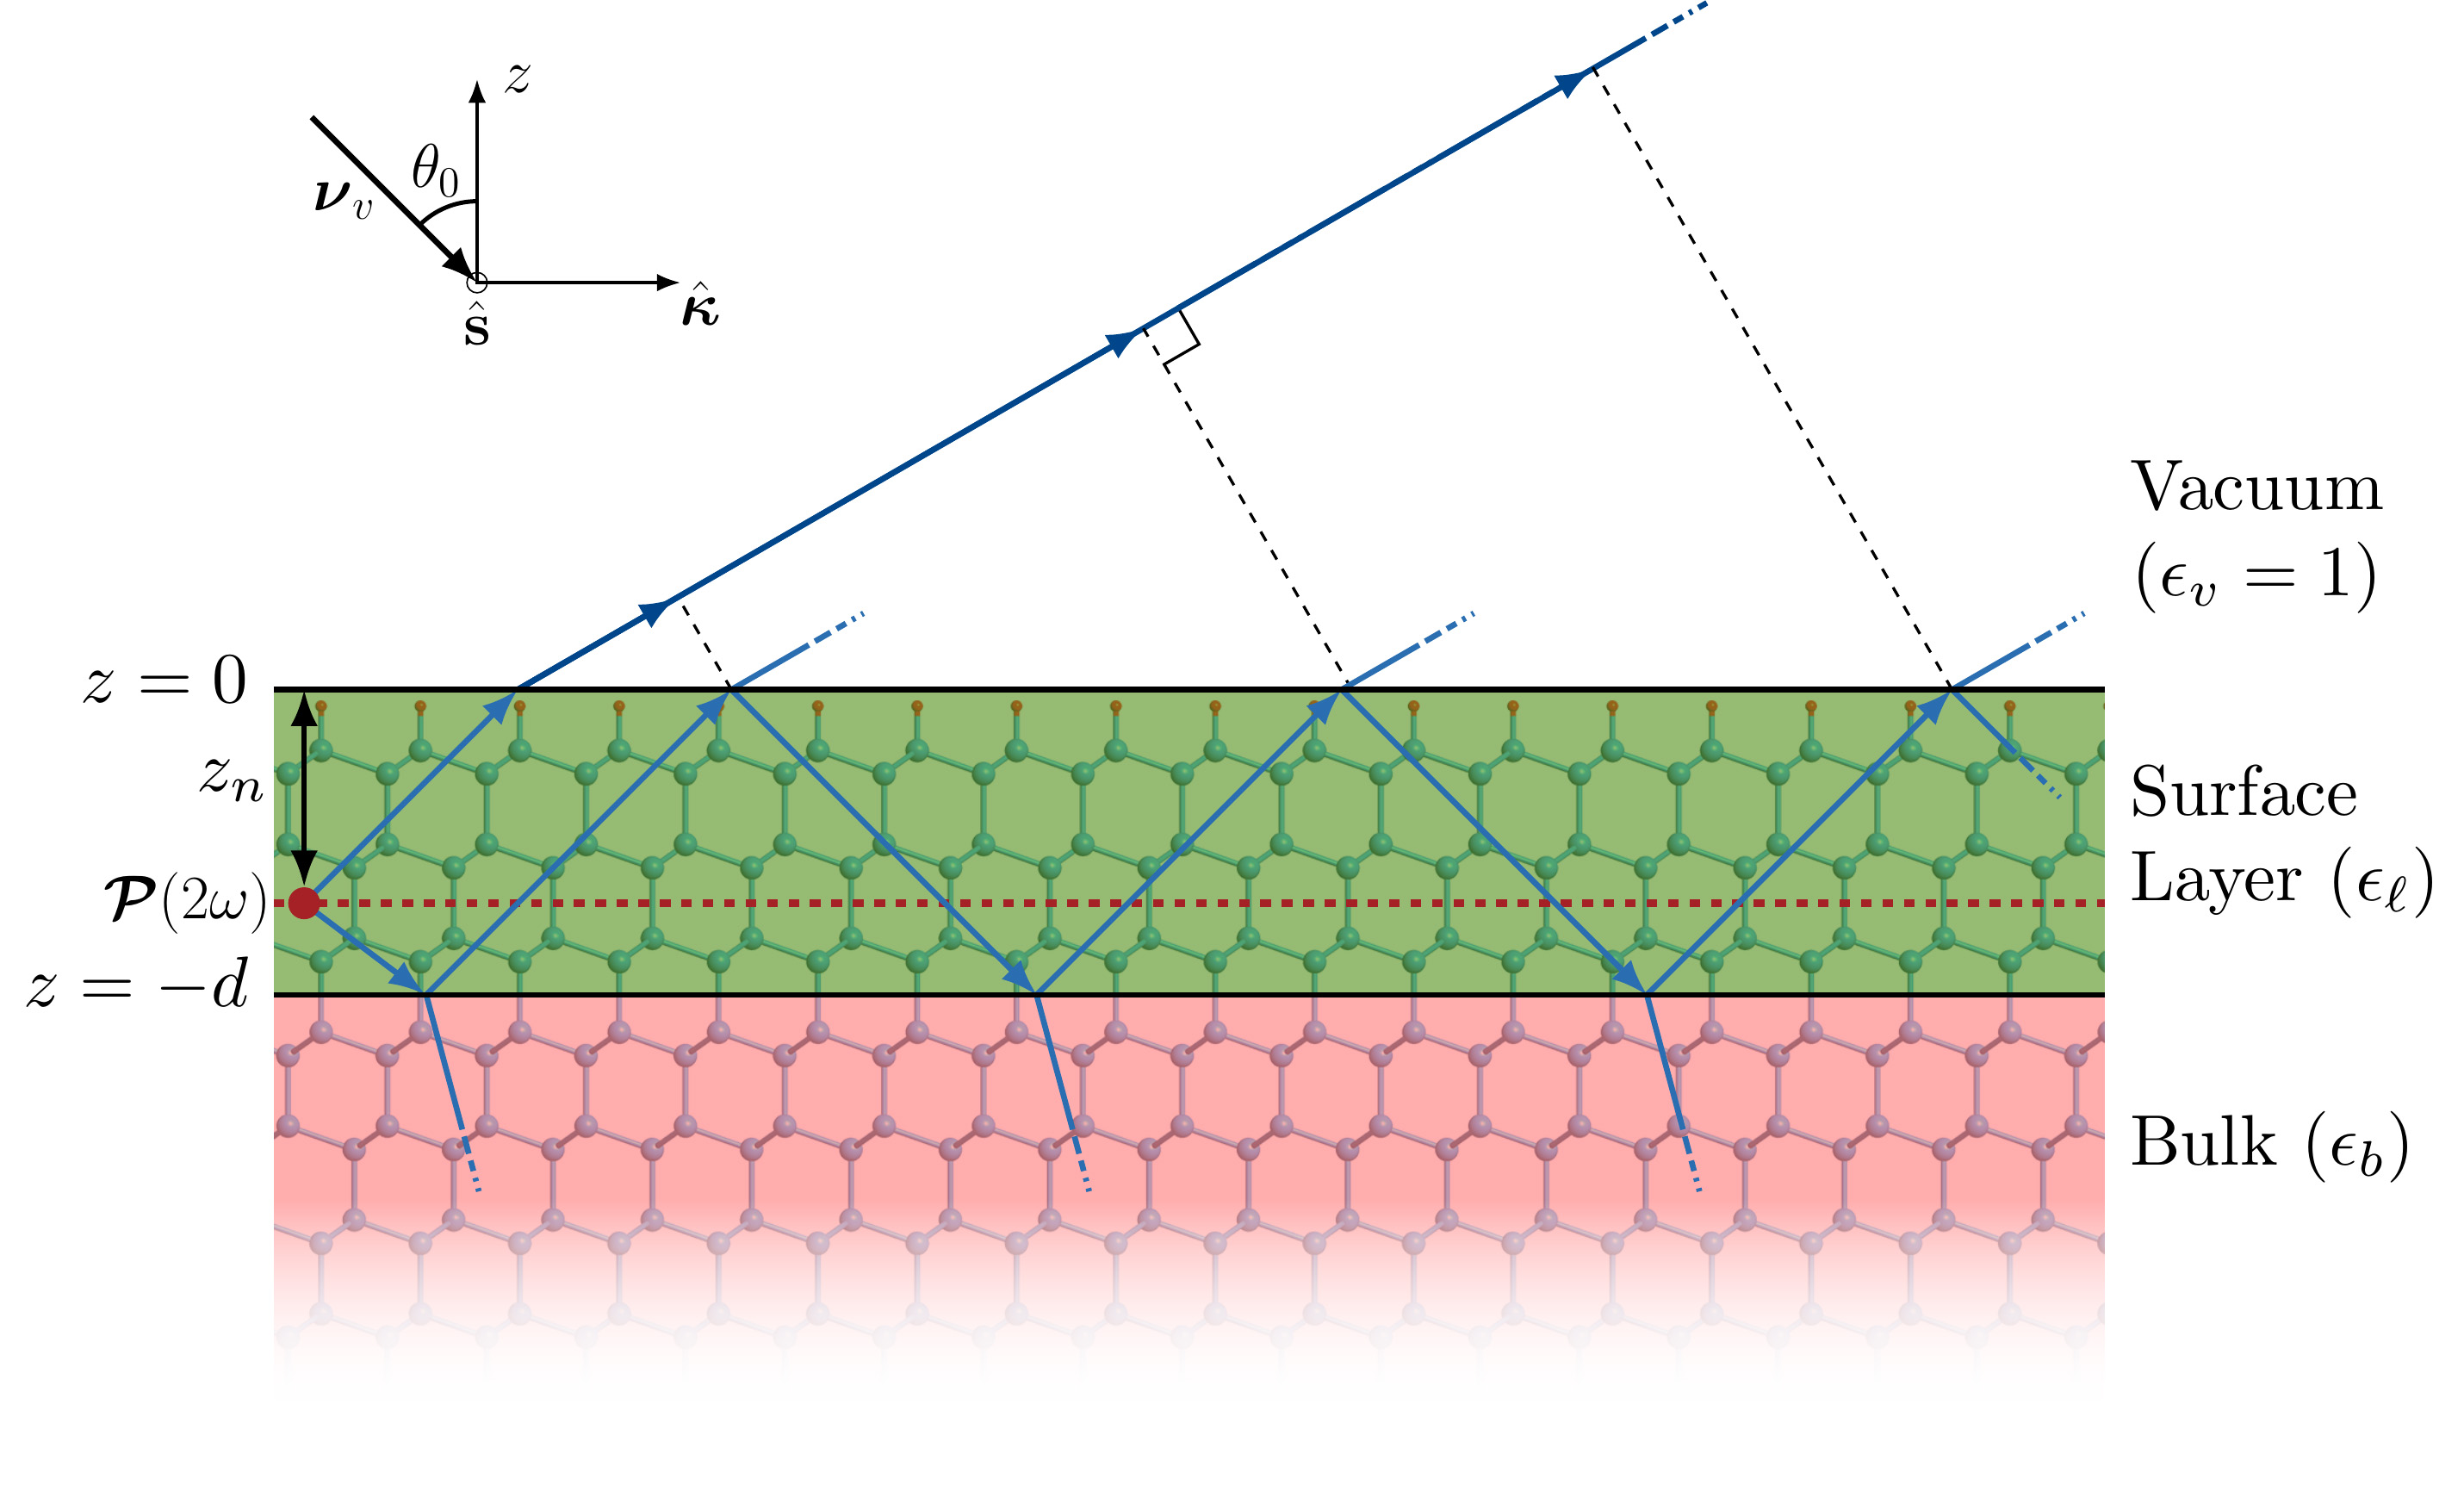
\includegraphics[width=0.7\textwidth]{fig1}
\caption{(Color online) Sketch of the three layer model for SHG. The vacuum
region ($v$) is on top with $\epsilon_{v}=1$; the layer $\ell$ of thickness $d$,
is characterized by $\epsilon_{\ell}(\omega)$, and it is where the SH
polarization sheet $\boldsymbol{\mathcal{P}}_{\ell}(2\omega)$ is located at a
distance $z_{n}$. The bulk $b$ is described by $\epsilon_{b}(\omega)$. The blue
lines within the slab represent the SH multiple reflections. The
Si(111)(1$\times$1):H surface is represented by the ball and stick model (H:
small spheres, Si: large spheres) in the background. The red dotted line is the
one of the many possible $z_{n}$ positions.}
\label{fig:MR3layer2w}
\end{figure}

\begin{figure}[b]
\centering 
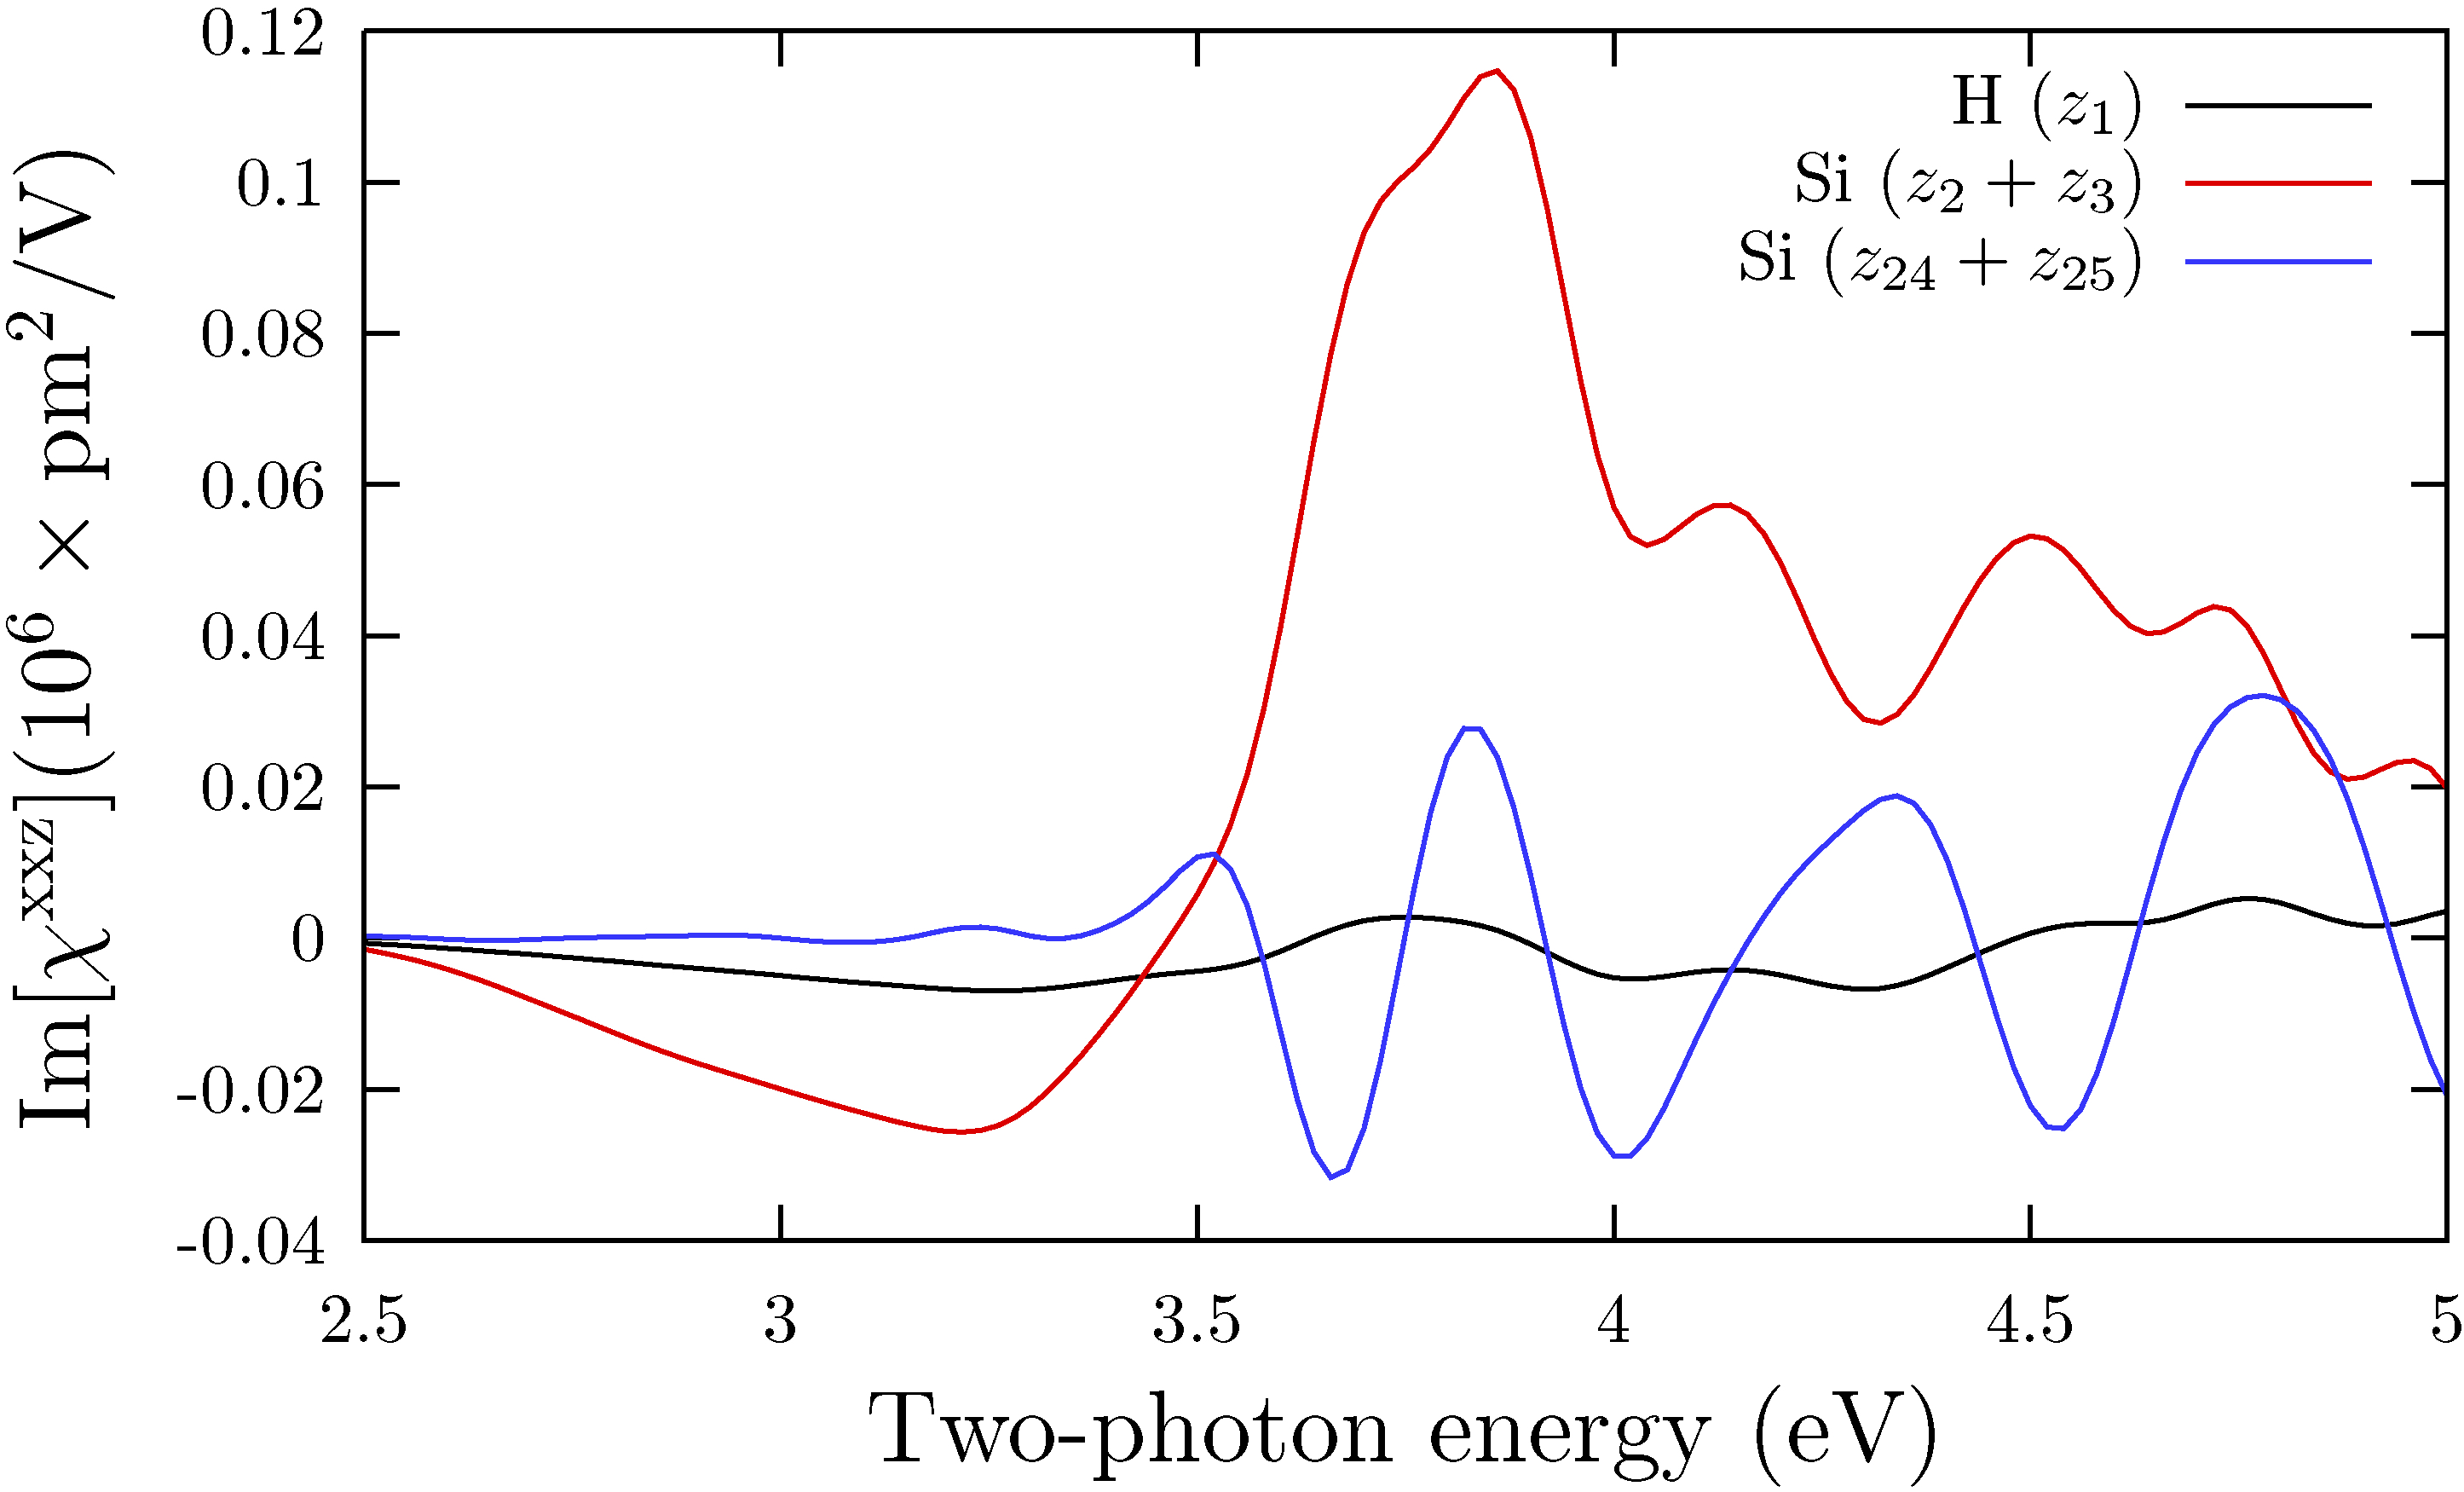
\includegraphics[width=0.6\textwidth]{fig2}
\caption{(Color online) 
Imaginary part of $\chi^{xxz}(z_{n})$ for the H layer ($z_1$), the sum of the
two topmost Si layers ($z_{2} + z_{3}$), and the sum of the bottommost Si layers
($z_{24 }+ z_{25}$) for the 25 layer half-slab used in this work.}
\label{fig2}
\end{figure}

\begin{figure}[b]
\centering 
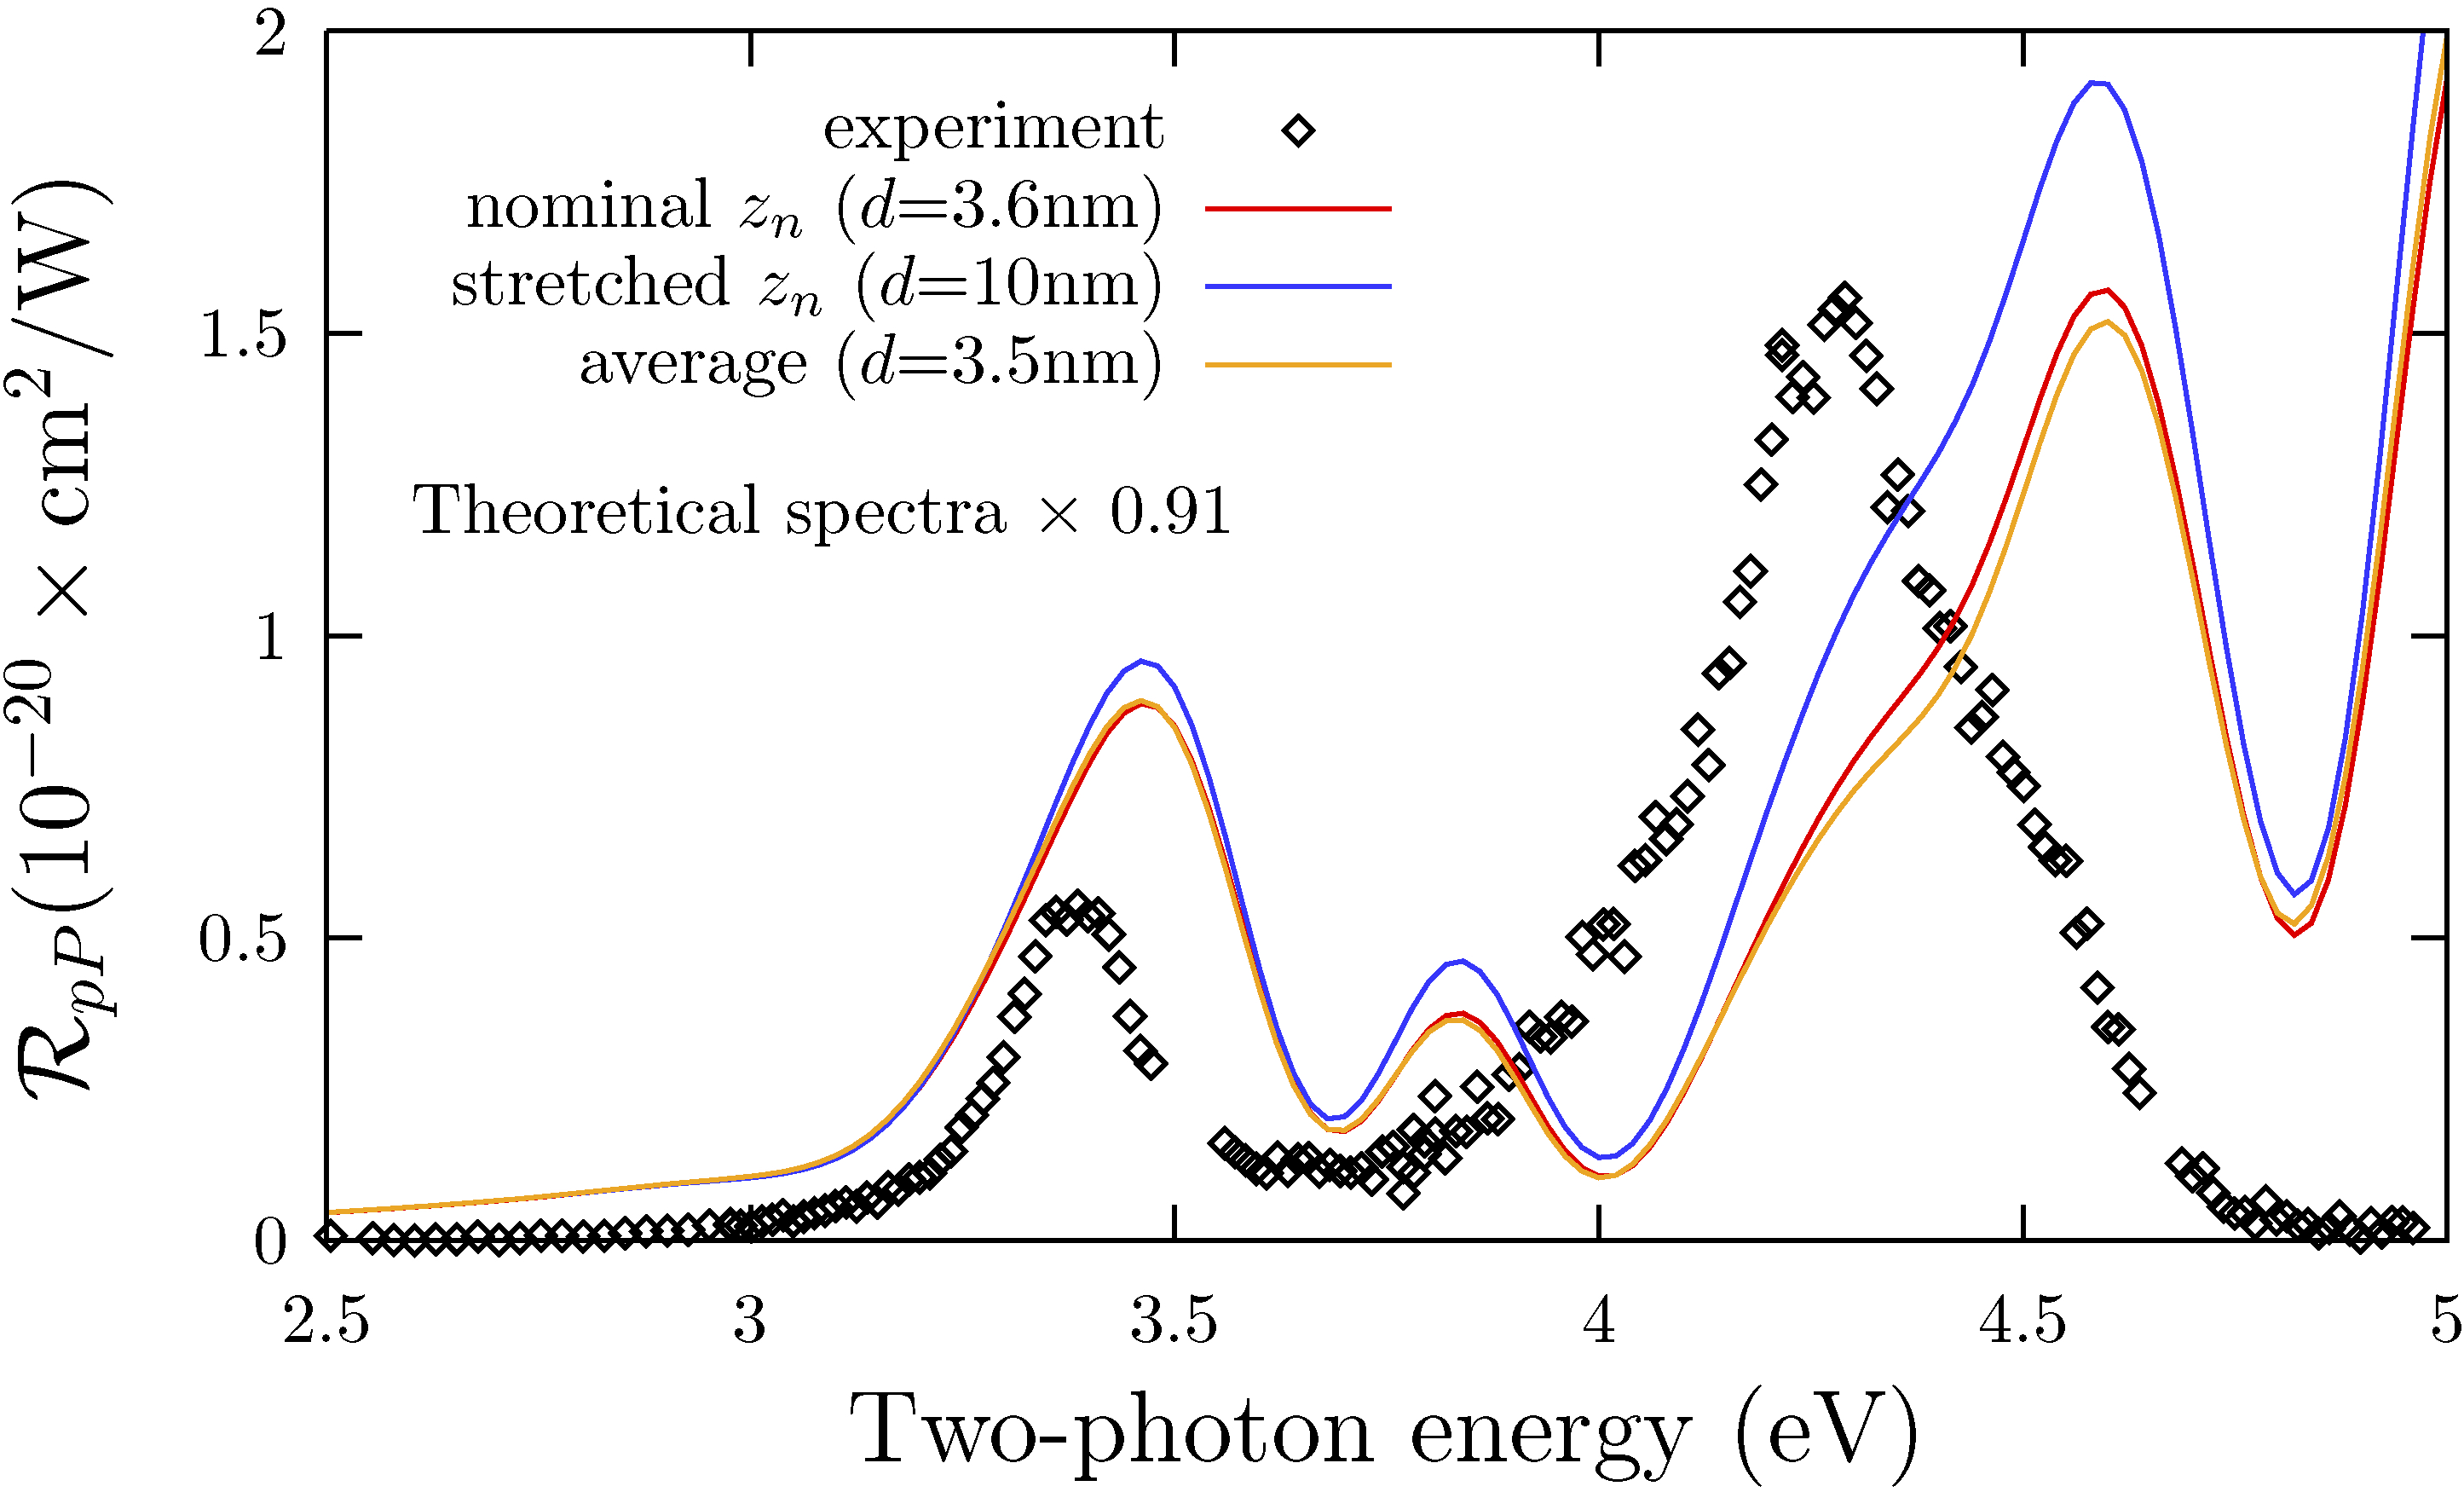
\includegraphics[width=0.6\textwidth]{fig3}
\caption{(Color online) $\mathcal{R}_{pP}$ for $z_{n}$ as given by the slab
(nominal, red line), $z_{n}$ stretched by 2.7 (stretched, blue line), and using
the half-slab value of $\chi^{\mathrm{abc}}_{\mathrm{hs}}$ (average, yellow
line), see text for details. The experimental data is from \cite{mejiaPRB02}. We
use $\theta = 65\,^{\circ}$, $\phi = 30\,^{\circ}$, and a broadening of $\sigma
= 0.075$ eV.}
\label{fig3}
\end{figure}

\end{document}
